\documentclass[../informe_krapp.tex]{subfiles}
\begin{document}
\section{Partes del proyecto}

\subsection{DOIT ESP32 DevKit v1}
\begin{wrapfigure}{r}{0in}
	\centering
	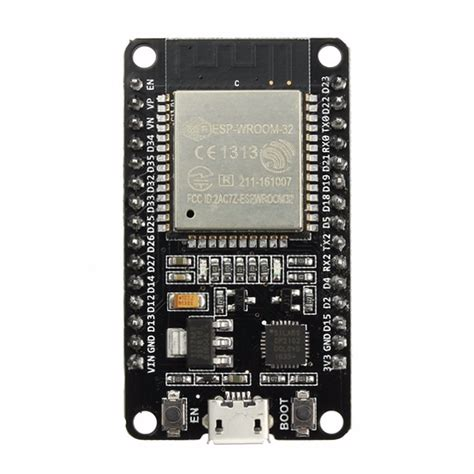
\includegraphics[width= 1.5in, keepaspectratio]{ESP32-board.jpg}
\end{wrapfigure}
El kit de desarrollo DOIT ESP32 DevKit v1 es una de las placas de desarrollo creadas por
DOIT. Esta basada en el microcontrolador ESP32, que en un mismo chip tiene soporte
para WiFi, Bluetooth, Ethernet y Low-Power

\subsubsection{Características Técnicas}
\begin{itemize}
	\item Microcontrolador: Tensilica 32-bit Single/Dual-core CPU Xtensa LX6
	\item Tensión de operación: 3.3V
	\item Tensión de alimentación: 7-12V
	\item Pines I/O digitales (DIO): 25
	\item Pines analógicos de Entrada (ADC): 6
	\item Pines analógicos de Salida (DAC): 2
	\item UARTs: 3
	\item SPIs: 2
	\item I2Cs: 3
	\item Memoria Flash: 4 MB
	\item SRAM: 520 KB
	\item Velocidad de clock: 240 Mhz
	\item Wi-Fi: IEEE 802.11 b/g/n/e/i, con las siguientes características:
	      \begin{itemize}
		      \item Switch TR, Balun, LNA, Amplificador de potencia y antena integrados
		      \item Autenticación WEP, WPA/WPA2, con la opcion de tambien acceder a redes abiertas.
	      \end{itemize}
\end{itemize}


\begin{figure}[H]
	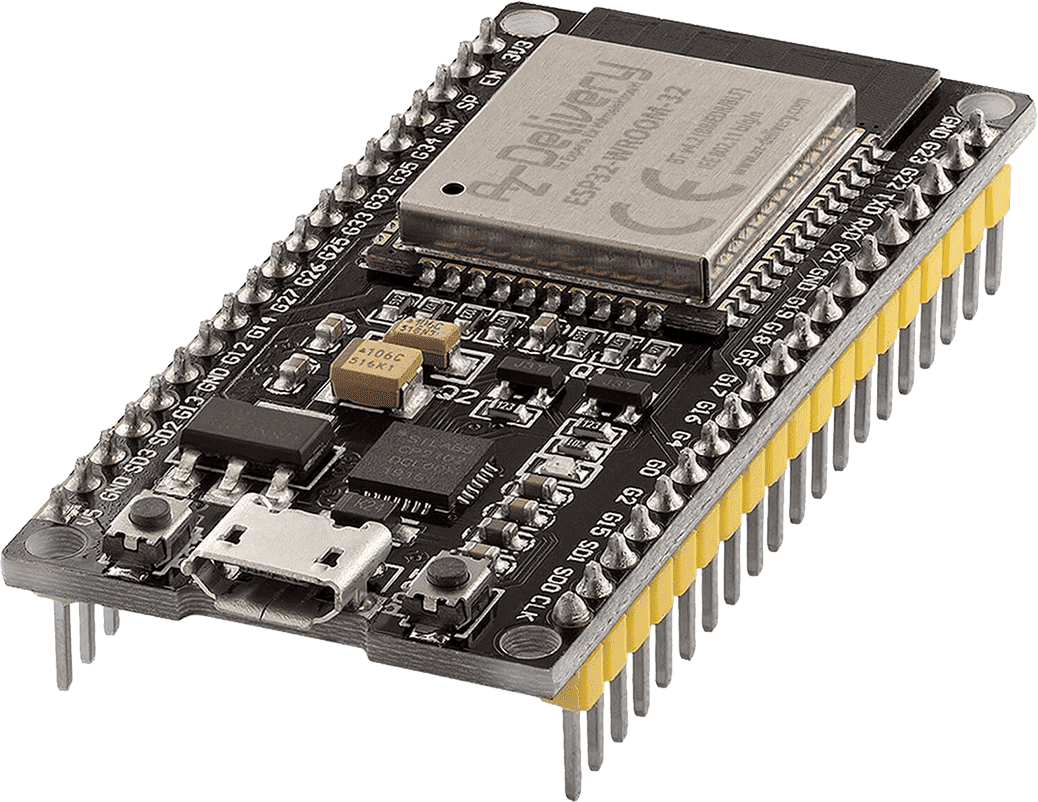
\includegraphics[width=0.55\textwidth]{esp32-2.png}
	\centering
	\caption{La placa DOIT DevKit ESP32}
\end{figure}

\clearpage

\subsubsection{Pinout}
\begin{figure}[H]
	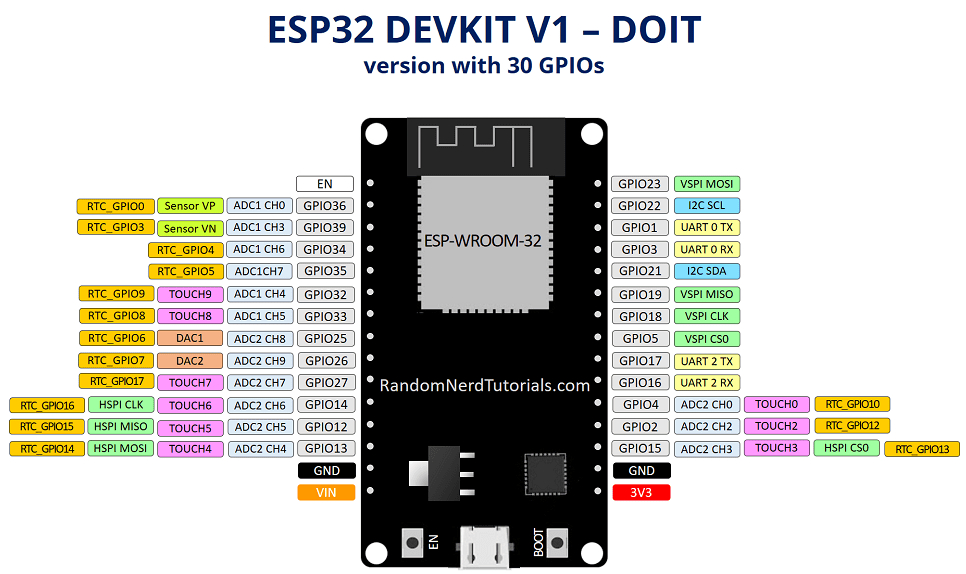
\includegraphics[width=0.85\textwidth]{ESP32-board-30pin-pinout.jpg}
	\centering
	\caption{Pinout de la placa de desarrollo DOIT DevKit V1 ESP32 de 30 pines}
\end{figure}

\begin{figure}[H]
	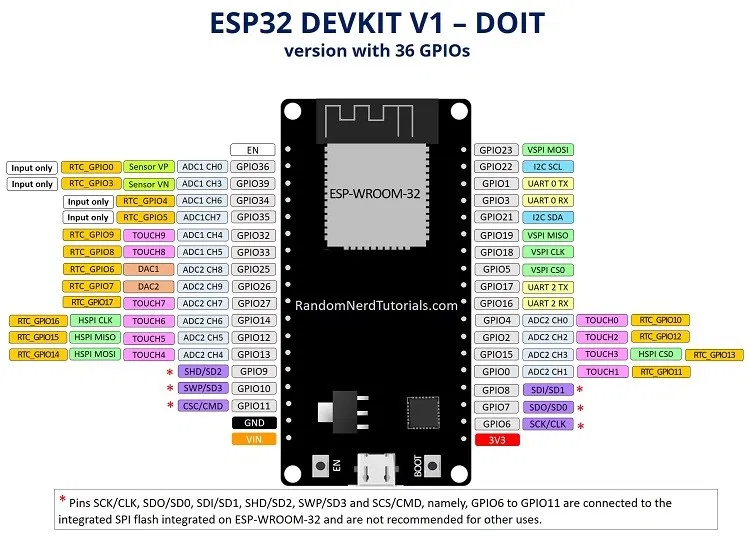
\includegraphics[width=0.85\textwidth]{ESP32-board-36pin-pinout.jpg}
	\centering
	\caption{Pinout de la placa de desarrollo DOIT DevKit V1 ESP32 de 36 pines,
		cabe recordar que los pines GPIO 6-11 estan reservados al sistema SPI integrado, y su
		uso no es recomendado}
\end{figure}
\subsubsection{Usabilidad de pines}
El ESP32 cuenta con una multitud de pines, pero no todos pueden ser usados libremente,
esto es explicado en la tabla \ref{tabla-pines-esp32} que muestra que pines pueden ser utilizados y cuales no,
dependiendo de las cirscuntancias.

A la hora de ser usados en el codigo c++ del framework Arduino, simplemente se refieren
por el numero

\begin{table}[!ht]
	\centering
	\begin{tabular}{|l|l|l|l|}
		\hline
		GPIO & Input     & Output & Notes                                      \\ \hline
		0    & pulled up & OK     & Hace output de señal PWM al arranque       \\ \hline
		1    & TX pin    & OK     & debug output al arranque                   \\ \hline
		2    & OK        & OK     & Conectado al LED\_ONBOARD                  \\ \hline
		3    & OK        & RX pin & En estado HIGH al arranque                 \\ \hline
		4    & OK        & OK     & ~                                          \\ \hline
		5    & OK        & OK     & Hace output de señal PWM al arranque       \\ \hline
		6    & x         & x      & Conectado al flash SPI integrado           \\ \hline
		7    & x         & x      & Conectado al flash SPI integrado           \\ \hline
		8    & x         & x      & Conectado al flash SPI integrado           \\ \hline
		9    & x         & x      & Conectado al flash SPI integrado           \\ \hline
		10   & x         & x      & Conectado al flash SPI integrado           \\ \hline
		11   & x         & x      & Conectado al flash SPI integrado           \\ \hline
		12   & OK        & OK     & El arranque falla si está pulleado en HIGH \\ \hline
		13   & OK        & OK     & ~                                          \\ \hline
		14   & OK        & OK     & Hace output de señal PWM al arranque       \\ \hline
		15   & OK        & OK     & Hace output de señal PWM al arranque       \\ \hline
		16   & OK        & OK     & ~                                          \\ \hline
		17   & OK        & OK     & ~                                          \\ \hline
		18   & OK        & OK     & ~                                          \\ \hline
		19   & OK        & OK     & ~                                          \\ \hline
		21   & OK        & OK     & ~                                          \\ \hline
		22   & OK        & OK     & ~                                          \\ \hline
		23   & OK        & OK     & ~                                          \\ \hline
		25   & OK        & OK     & ~                                          \\ \hline
		26   & OK        & OK     & ~                                          \\ \hline
		27   & OK        & OK     & ~                                          \\ \hline
		32   & OK        & OK     & ~                                          \\ \hline
		33   & OK        & OK     & ~                                          \\ \hline
		34   & OK        & x      & Solamente de input                         \\ \hline
		35   & OK        & x      & Solamente de input                         \\ \hline
		36   & OK        & x      & Solamente de input                         \\ \hline
		39   & OK        & x      & Solamente de input                         \\ \hline
	\end{tabular}
	\caption{Una tabla con las funciones de cada pin de la placa de desarrollo
		DOIT DevKit v1 ESP32}
	\label{tabla-pines-esp32}
\end{table}

\clearpage
\subsection{Sistema RFID}
Segun Wikipedia\cite{wikipedia_rfid_es}:

\begin{center}
	\rule{0.8\textwidth}{0.3pt}
\end{center}
``RFID o identificación por radiofrecuencia
(del inglés Radio Frequency Identification) es un sistema de almacenamiento y recuperación
de datos remotos que usa dispositivos denominados etiquetas, tarjetas o transpondedores
RFID.

\begin{wrapfigure}{r}{0in}
	\centering
	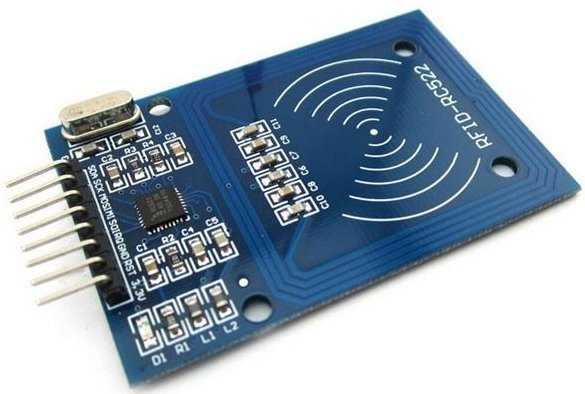
\includegraphics[width= 1.5in, keepaspectratio]{rfid-rc552.jpg}
\end{wrapfigure}

El propósito fundamental de la tecnología RFID es transmitir la identidad de
un objeto (similar a un número de serie único) mediante ondas de radio. Las tecnologías
RFID se agrupan dentro de las denominadas Auto ID (automatic identification,
o identificación automática).

Las etiquetas RFID (RFID tag en inglés) son unos dispositivos pequeños, similares
a una pegatina, que pueden ser adheridas o incorporadas a un producto, un animal
o una persona. Contienen antenas para permitirles recibir y responder a peticiones
por radiofrecuencia desde un emisor-receptor RFID. Las etiquetas pasivas no necesitan
alimentación eléctrica interna, mientras que las activas sí lo requieren.

Una de las ventajas del uso de radiofrecuencia (en lugar, por ejemplo, de infrarrojos)
es que no se requiere visión directa entre emisor y receptor''

\begin{center}
	\rule{0.8\textwidth}{0.3pt}
\end{center}

\begin{figure}[H]
	\centering
	\begin{subfigure}{0.4\textwidth}
		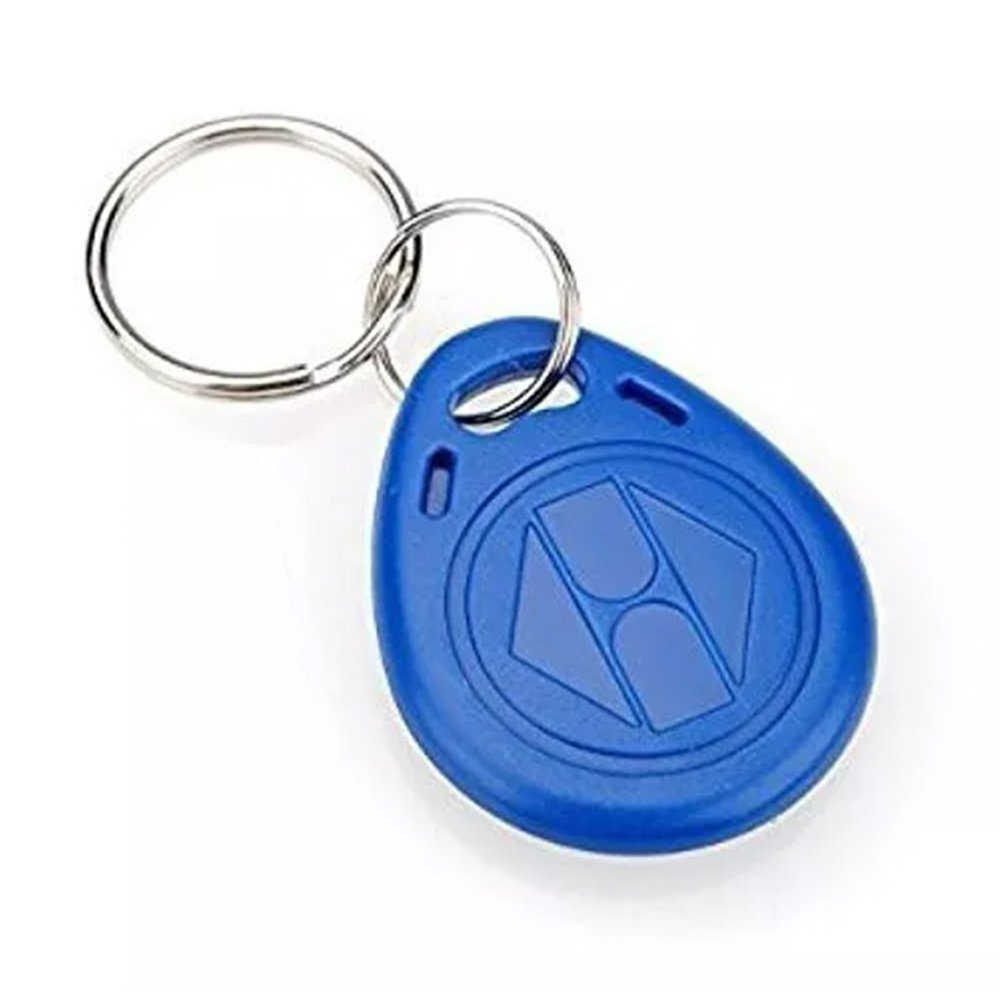
\includegraphics[width=0.7\textwidth]{llavero-rfid.jpg}
		\caption{Un llavero RFID}
	\end{subfigure}
	\begin{subfigure}{0.4\textwidth}
		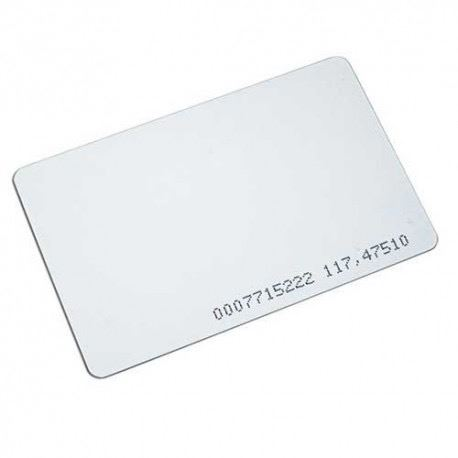
\includegraphics[width=0.7\textwidth]{tarjeta-rfid.jpg}
		\caption{Una tarjeta RFID}
	\end{subfigure}
	\caption{Distintos tags RFID}
\end{figure}

\clearpage
\subsubsection{Pinout del dispositivo}

\begin{wrapfigure}{r}{0in}
	\centering
	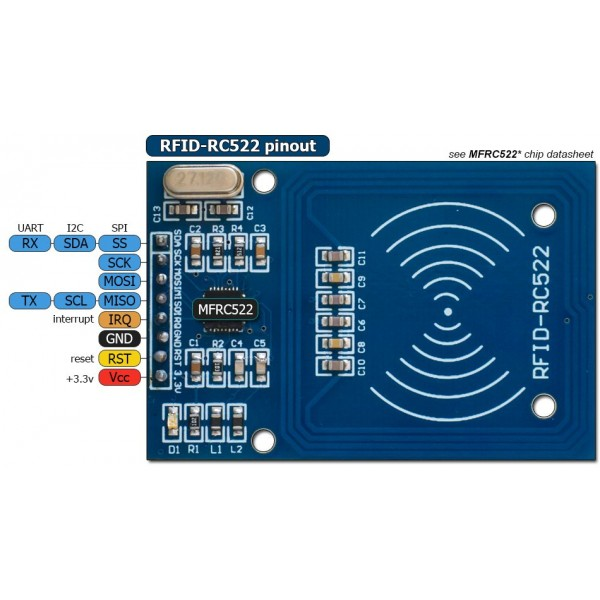
\includegraphics[width=0.5\textwidth]{rfid-rc522-pinout.jpg}
	\caption{El pinout del lector RFID-RC552.
		Se puede notar como este dispositivo está adaptado para funcionar con 3 protocolos
		distintos, comunicación por UART, comunicación por I2C y comunicacion por SPI}
\end{wrapfigure}

% la verdad es que este "---" esta RE mal, lo tendria que cambiar con titlesec

\paragraph{pin SDA ---}
Este pin se utiliza de forma distinta dependiendo del protocolo
de comunicación utilizado.
\begin{itemize}
	\item En I2C, se usa como el pin SDA.
	\item En UART, se usa como pin RX.
	\item En SPI, se usa como el pin SS
\end{itemize}

\paragraph{pin SCK ---}
El pin SCK se usa para mantener el sincronísmo con una señal de reloj

\paragraph{pin MOSI ---}
El pin MOSI sirve para hacer una transmisión Master Out - Slave In

\paragraph{pin MISO ---}
El pin MISO sirve para hacer una transmisión Master In - Slave Out

\paragraph{pin IRQ ---}
Se usa para las interrupciones

\paragraph{GND ---}
Sirve para mantener la referencia con Masa

\paragraph{RST ---}
Este pin sirve para resetear o desactivar el circuito integrado

\paragraph{VCC ---}
Pin de alimentación \textbf{3.3v}

\clearpage
\subsubsection{Mapeo de Memoria del tag RFID}
La identificación se realiza con unos llaveros o unas tarjetas,
que tienen este mapeo de memoria:

Tenemos 1k de memoria adentro de este chip, la cual esta organizada de la
siguiente manera: Hay 16 sectores de 4 bloques, y cada bloque contiene 16 bytes.

\begin{figure}[H]
	\centering
	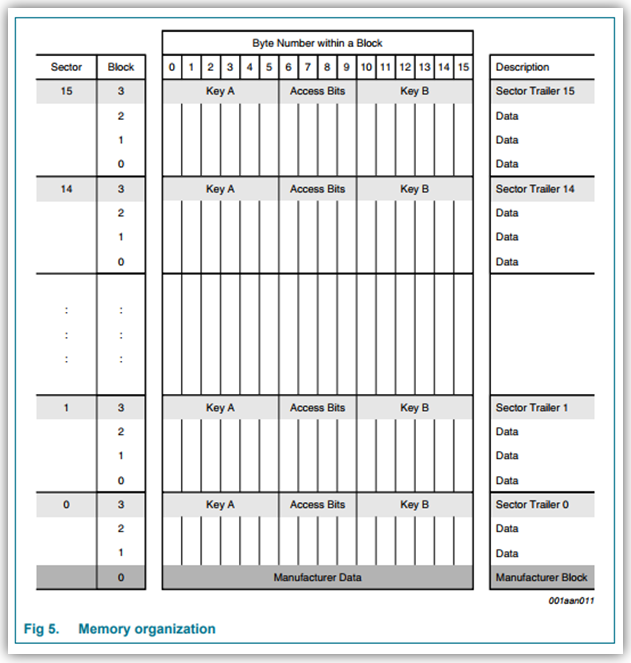
\includegraphics[width=0.9\textwidth]{rfid-mapeo-memoria.png}
\end{figure}

\clearpage

\subsection{Pantalla OLED SSD1306}
Las pantallas OLED se tratan de pantallas que utilizan diodos LED orgánicos capaces de consumir muy poca energía.
Estas pantallas son muy delgadas, se comunican por I2C o SPI y producen una imagen más brillante y nítida que los típicos display LCD.

OLED son las siglas en inglés de Organic Light-Emitting Diode que traducido al español sería diodo orgánico de emisión de luz.

\begin{figure}[H]
	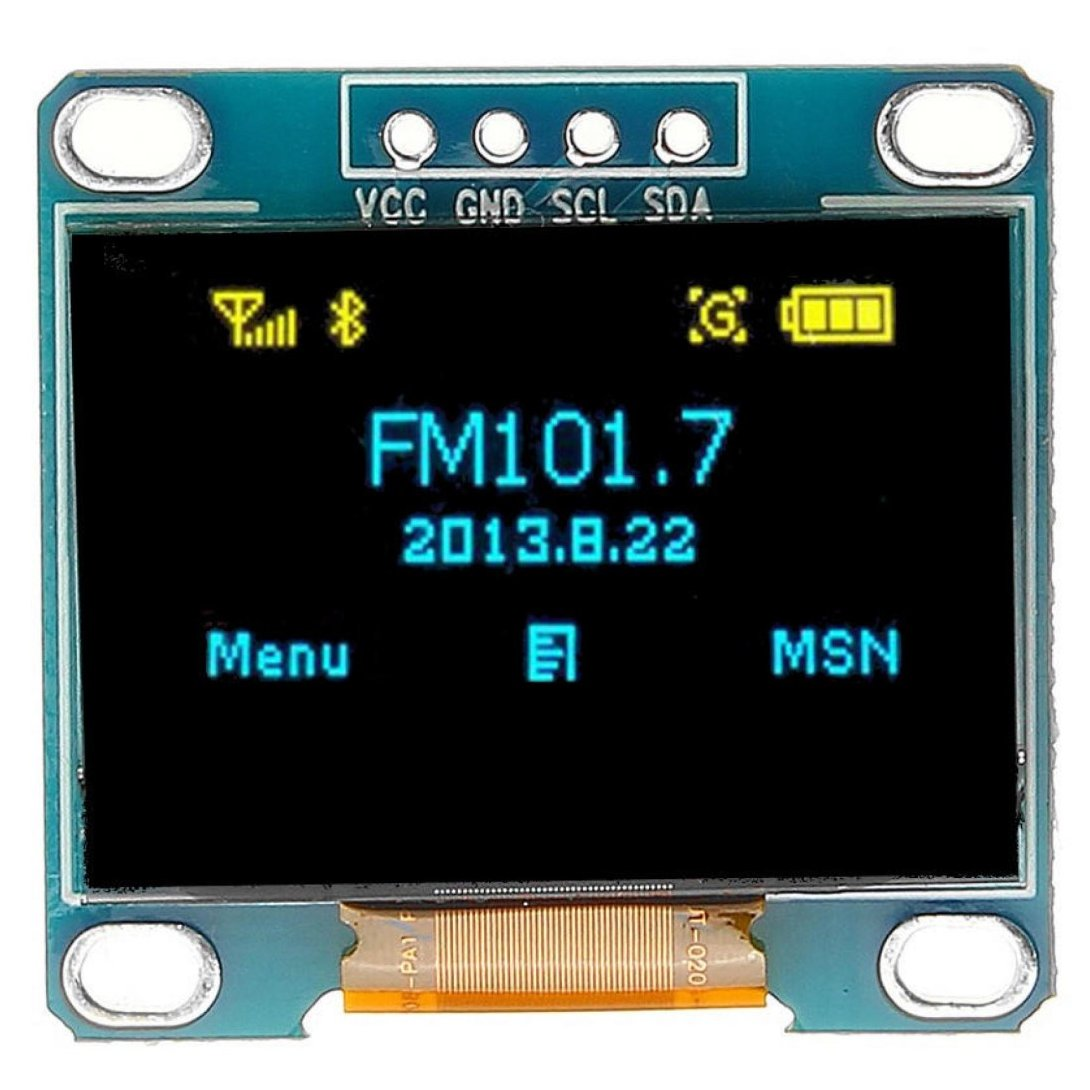
\includegraphics[width=0.4\textwidth, keepaspectratio]{oled}
	\centering
\end{figure}

Las pantallas OLED están compuestas por láminas de materiales orgánicos como el carbón (por eso el nombre de diodo orgánico). Estas láminas emiten luz cuando se les aplica electricidad entre ellas.

Una de las ventajas de las pantallas OLED con respecto a pantalla LCD es que no requieren de una luz de fondo ni de filtros. Esto hace que las pantallas OLED sean más eficientes en términos de energía, más fáciles de fabricar y mucho más finas. A parte pueden ser flexibles y transparentes.

\begin{figure}[H]
	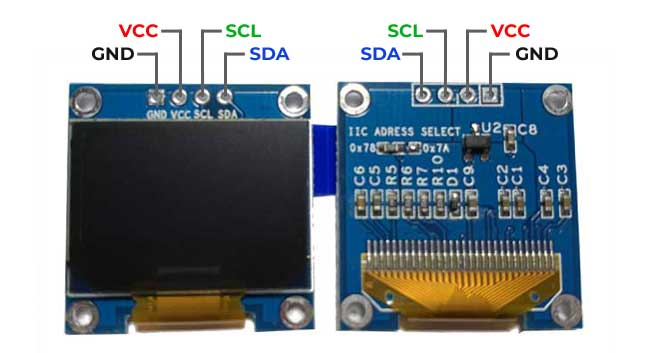
\includegraphics[width=0.7\textwidth, keepaspectratio]{oled-pinout}
	\centering
	\caption{Pinout del dispositivo}
\end{figure}

\end{document}
